%\documentclass[envcountsect,handout]{beamer}
\documentclass[envcountsect]{beamer}
\setbeamertemplate{theorems}[numbered]
\usetheme{Boadilla}

% Tikz graphics - should these be imported as images instead?
\usepackage{graphicx, tikz}
\usetikzlibrary{shapes, arrows, positioning, calc}

\usepackage{multirow}
\usepackage{mathtools}
\DeclareMathOperator*{\argmax}{arg\,max}

\title{Introduction to Part-of-Speech Tagging}
\subtitle{Basic Graphical Models for Sequence Labelling}
\author{Alex Simcock}
\institute{University of Birmingham}
\date{\today}

\begin{document}

\begin{frame}
\titlepage
\end{frame}

\begin{frame}{Part-of-Speech Tagging}

\begin{definition}[Part-of-Speech]
The term `part-of-speech' refers to the syntactic category of a word, for example noun, verb or adjective.
\end{definition}

\begin{example}[Ambiguous Parts-of-Speech]
\begin{center}
\begin{tabular}{ c c c c c }
 `The & fans & watch & the & race' \\
 \hline
 \textbf{Dt} & \textbf{Nn} & \textbf{Nn} & \textbf{Dt} & \textbf{Nn} \\  
 & \textbf{Vb} & \textbf{Vb} & & \textbf{Vb}    
\end{tabular}
\end{center}
\end{example}

How can we best label any given word sequence in the presence of grammatical-ambiguity?

%Part-of-speech tagging is a key preliminary step in many natural language processing pipelines.

\end{frame}

\begin{frame}

\begin{definition}[POS Tagging as Structure Prediction]

Let $X$ and $Y$ be random variables such that $X$ varies over all word sequences and $Y$ over all label sequences.

\begin{align*}
    X &= (x_k)_{k=1}^n = (\text{`the'}, \text{`fans'}, \text{`watch'}, \text{`the'}, \text{`race'}) \\
    Y &= (y_k)_{k=1}^n = (\textbf{Dt}, \textbf{Nn}, \textbf{Nn}, \textbf{Dt}, \textbf{Nn}), \quad y_k \in \mathcal{Y}
\end{align*}

The POS tagging problem can now be written:

`\textbf{Given $X$, predict the correctly matched tag sequence $Y$}'.

\end{definition}

%\pause

\textbf{Maximum likelihood estimation} tells us that the best choice of $Y$ will maximise the probability of observing our word sequence:
\begin{equation*}
    Y^* \coloneqq \argmax_{Y} p(Y \mid X)
\end{equation*}    

\end{frame}

\begin{frame}{The Na{\"i}ve Bayes Classifier}

\begin{definition}[Na{\"i}ve Bayes Classifier]
    Na{\"i}ve Bayes models the joint probability distribution $p(X,Y)$:
    \begin{equation*}
        p(X,Y) = \prod_{i=1}^n p(X_i \mid Y_i)p(Y_i)
    \end{equation*}
\end{definition}

We can apply the Na{\"i}ve Bayes model to derive $Y^*$,
\begin{gather*}
    p(Y \mid X) = \frac{p(Y,X)}{p(X)} = \frac{1}{p(X)}\prod_{i=1}^n p(X_i \mid Y_i)p(Y_i) = \frac{1}{p(X)}\prod_{i=1}^n p(X_i, Y_i) \\
    \therefore Y^* = \argmax_Y p(Y \mid X) = \argmax_Y \prod_{i=1}^n p(X_i, Y_i)
\end{gather*}

The result is a model which simply selects the most common tag for each word!
%Despite the simplicity of this approach the accuracy rate is likely to be high: many words have only one appropriate syntactic category.

\end{frame}

\begin{frame}%{Na{\"i}ve Bayes as a Graphical Model}

\begin{figure}[ht]
\centering
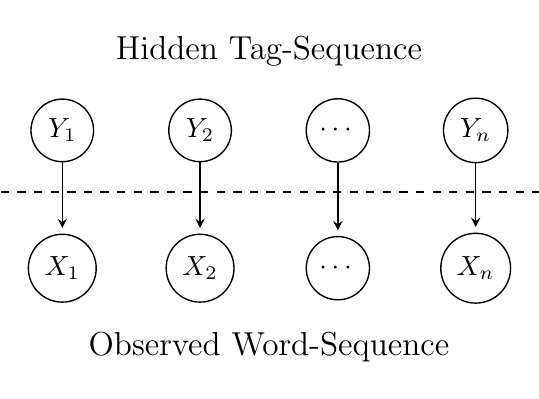
\begin{tikzpicture} [-> , >= stealth, shorten >= 2 pt, line width = 0.5pt, node distance = 1.75cm]

\node [draw, circle] (y1) {$Y_1$};
\node [draw, circle] (y2) [right of = y1] {$Y_2$};
\node [draw, circle] (ydot) [right of = y2] {$\cdots$};
\node [draw, circle] (yn) [right of = ydot] {$Y_n$};

\node [draw, circle] (x1) [below of = y1] {$X_1$};
\node [draw, circle] (x2) [below of = y2] {$X_2$};
\node [draw, circle] (xdot) [below of = ydot] {$\cdots$};
\node [draw, circle] (xn) [below of = yn] {$X_n$};

\path (y1) edge (x1);
\path (y2) edge (x2);
\path (ydot) edge (xdot);
\path (yn) edge (xn);


\node (c1w1) at ($(y1)!0.45!(x1)$) {};
\node (c3w3) at ($(yn)!0.45!(xn)$) {};
\draw [-, dashed, line width =0.75 pt, shorten >=-1.75cm, shorten <=-1.75cm] (c1w1) -- (c3w3);

\node (y2.5) at ($(y2)!0.5!(ydot)$) {};
\node (x2.5) at ($(x2)!0.5!(xdot)$) {};
\node [above of = y2.5, node distance= 1cm] {\large Hidden Tag-Sequence};
\node [below of = x2.5, node distance= 1cm] {\large Observed Word-Sequence};

\end{tikzpicture}
\end{figure}

\end{frame}

\begin{frame}{The Hidden Markov Model (HMM)}

\begin{figure}[ht]
\centering
\hspace{-1.9cm}
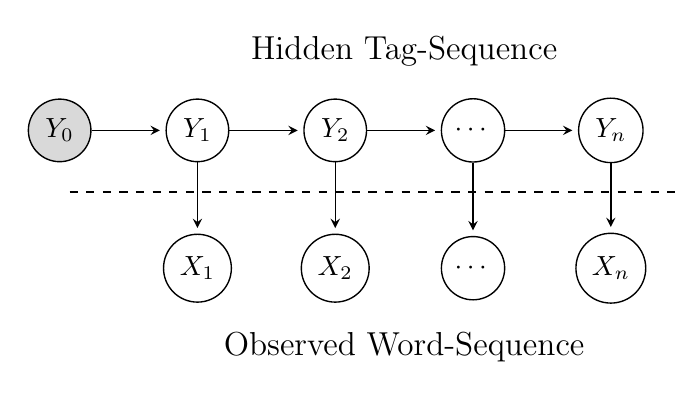
\begin{tikzpicture} [-> , >= stealth, shorten >= 2 pt, line width = 0.5pt, node distance = 1.75cm]

\node [draw, circle] (y1) {$Y_1$};
\node (start) [draw, circle, fill=gray!30!white, left of = y1] {$Y_0$};
\node [draw, circle] (y2) [right of = y1] {$Y_2$};
\node [draw, circle] (ydot) [right of = y2] {$\cdots$};
\node [draw, circle] (yn) [right of = ydot] {$Y_n$};

\path (start) edge (y1);
\path (y1) edge (y2);
\path (y2) edge (ydot);
\path (ydot) edge (yn);

\node [draw, circle] (x1) [below of = y1] {$X_1$};
\node [draw, circle] (x2) [below of = y2] {$X_2$};
\node [draw, circle] (xdot) [below of = ydot] {$\cdots$};
\node [draw, circle] (xn) [below of = yn] {$X_n$};

\path (y1) edge (x1);
\path (y2) edge (x2);
\path (ydot) edge (xdot);
\path (yn) edge (xn);


\node (c1w1) at ($(y1)!0.45!(x1)$) {};
\node (c3w3) at ($(yn)!0.45!(xn)$) {};
\draw [-, dashed, line width =0.75 pt, shorten >=-1.75cm, shorten <=-1.75cm] (c1w1) -- (c3w3);

\node (y2.5) at ($(y2)!0.5!(ydot)$) {};
\node (x2.5) at ($(x2)!0.5!(xdot)$) {};

\node [above of = y2.5, node distance= 1cm] {\large Hidden Tag-Sequence};
\node [below of = x2.5, node distance= 1cm] {\large Observed Word-Sequence};

\end{tikzpicture}
\end{figure}

\end{frame}

\begin{frame}

Like the NB the HMM is \textbf{generative}, which means we can understand the assumptions it makes by the generative story it tells:
\begin{enumerate}
    \item First, the hidden sequence $Y$ is generated by a walk over the Markov chain on $\mathcal{Y}$.
    \item At each node $Y_k$ visited on the walk, a word is drawn (according to $Y_k$'s distribution) and appended to $X$.
\end{enumerate}

%\pause

The HMM can be summarised by its key parameters, the sets of emission and transition probabilities: $A$ and $B$.
%(the probability of outputting a specified word given a specific tag)
%(the probability of traversing from one given tag to a specified tag)
%Note that transition from one node back into itself is permitted as long as an arc was traversed.
\begin{align*}
    A &= [ A_k(w) ] \quad k \in \mathcal{Y}, & \quad & A_k(w) = p(X_t = w \mid Y_t = k), \\
    B  &= [ B_{k,k'} ] \quad k, k' \in \mathcal{Y}, & \quad  & B_{k,k'} = p(Y_t = k' \mid Y_{t-1} = k), \\
    \pi &= [ \pi_k ] \quad k \in \mathcal{Y}, & \quad & \pi_k = p(Y_1 = k).
\end{align*}
%Point out places in diagram

\end{frame}

\begin{frame}

There are three key questions for HMMs:
\begin{enumerate}
    \item Given the observed sequence $X$ and a HMM $\theta = (A, B, \pi)$, how do we efficiently compute $p(X \mid \theta)$?
    \item \textbf{Given the observed sequence $X$ and a HMM $\theta = (A, B, \pi)$, how do we choose the corresponding state sequence $Y$ that best explains the observations?}
    \item How might we adjust the model parameters in order to maximise $p(X \mid \theta)$?
\end{enumerate}

\end{frame}

\begin{frame}{The Forward-Backward Algorithm}

%Answering part one...
%Derive equation
%Complexity so high
%the forward-backwad algorithm can be adapted to offer some unique practical applications of its own such as identifying the most likely author of a given text.

We can derive $p(X \mid \theta)$ by imagining all possible state-sequences $Y$, then finding all joint probabilities $p(X, Y \mid \theta)$ and finally summing these values back over all $Y$.
To do so we require two identities that result from the model assumptions of emission independence and markov property:
\begin{alignat*}{2}
    p(X \mid Y, \theta) &= \prod_{i=1}^n p(X_i \mid Y_i, \theta) = \prod_{i=1}^n A_{Y_i}(X_i) \\
    p(Y \mid \theta) &= \pi_{Y_1} B_{Y_1,Y_2} \cdots T_{Y_{n-1},Y_n}
\end{alignat*}
These identities can then be applied as follows,
\begin{align*}
    p(X \mid \theta) &= \sum_{\forall \: Y} p(X,Y \mid \theta) = \sum_{\forall \: Y} p(X \mid Y, \theta) p(Y \mid \theta) \\
    &= \sum_{\forall \: Y} \pi_{Y_1} A_{Y_1}(X_1) B_{Y_1, Y_2} A_{Y_2}(X_2) \cdots B_{Y_{n-1}, Y_n} A_{Y_n}(X_n)
\end{align*}

This calculation is intractable and has exponential complexity $O(2n|\mathcal{Y}|^n)$.
% owing to the $2n - 1$ multiplications for each of the $|\mathcal{Y}|^n$ possible values of $Y$.
%A model trained on the base tagset of the BNC ($|\mathcal{Y}|=61$) would require $7.99 \times 10^{19}$ calculations to calculate $p(X \mid \theta)$ for a sequence of only five words.

\end{frame}

\begin{frame}
    In order to calculate more efficiently we will use induction...
    \begin{definition}[Forward-Function]
        Let $\alpha_t(k)$ denote the joint probability of observing the sequence $X_1 X_2 \cdots X_t \, (1 \leq t \leq n$) and the tag $Y_t$ being $k$, given model parameters $\theta$.
        \begin{equation*}
            \alpha_t(k) \coloneqq p(X_1,X_2,\ldots,X_t,Y_t=k \mid \theta)
        \end{equation*}
    \end{definition}

Having defined $\alpha_t(k)$, we note that $p(X \mid \theta) = \sum_{k \in \mathcal{Y}} \alpha_n(k)$, if we can efficiently solve for a given $\alpha_t(k)$ then we have answered the first question!

The solution is the `forward-algorithm':
\begin{align*}
    \alpha_1(k) &= \pi_{k} A_k(X_1) & \quad & \:\: k \in \mathcal{Y} \\
    \alpha_{t+1}(k) &= \left[ \sum_{k' \in \mathcal{Y}} \alpha_{t}(k')B_{X_t,X_{t+1}} \right] A_k(X_{t+1}) & \quad &
        \begin{array}{lr}
            1 \leq t \leq n-1\\
            k, k' \in \mathcal{Y}
        \end{array}
\end{align*}
    
\end{frame}

\begin{frame}
    At each step of induction we calculate the value $\alpha_t$ for all $|\mathcal{Y}|$ states, where each is derived from $|\mathcal{Y}|$ previous states.
Carrying out this calculation for each of the $n-1$ steps results in overall complexity of order $O(n|\mathcal{Y}|^2)$.

Our earlier example `the fans watch the race' with the tagset of the bnc $|\mathcal{Y}|=61,n=5$ experiences a reduction in calculations from over $10^{15}$ times less.

The backward algorithm....


\end{frame}

\begin{frame}{The Viterbi Algorithm}
    
\end{frame}

\begin{frame}{Going Beyond}
    
\end{frame}

\begin{frame}
\begin{center}
    \huge Thank you for listening.
\end{center}
\end{frame}

\end{document}



\end{frame}

\begin{frame}

give the algorithm
Describe that the backward one is similar

Having defined $\alpha_t(k)$, we note that $\prob (X \mid \theta) = \sum_{k \in \mathcal{Y}} \alpha_n(k)$.
The value of $\alpha_t(k)$ can be found by the `forward-algorithm' which applies induction, starting at $t=1$ and repeatedly applying the inductive step (\ref{eq:forward-inductive}) until the desired value of $t$ is reached.

\begin{gather*}
    \text{Base Case:} \quad \alpha_1(k) = \pi_{k} E_{k,X_1} \qquad k \in \mathcal{Y} \\
    \text{Inductive Step:} \quad \alpha_{t+1}(k) = \left[ \sum_{k' \in \mathcal{Y}} \alpha_{t}(k')T_{X_t,X_{t+1}} \right] E_{k,X_{t+1}} \qquad
        \begin{array}{lr}
            1 \leq t \leq n-1\\
            k, k' \in \mathcal{Y}
        \end{array} \label{eq:forward-inductive}
\end{gather*}

At each step of induction we calculate the value $\alpha_t$ for all $|\mathcal{Y}|$ states, where each is derived from $|\mathcal{Y}|$ previous states.
Carrying out this calculation for each of the $n-1$ steps results in overall complexity of order $O(n|\mathcal{Y}|^2)$.
In real terms, the earlier example with parameters $|\mathcal{Y}|=61,n=5$ goes from over $7.99 \times 10^{19}$ calculations to $18605$. Most real-world examples will have much higher $n$ values and so savings in efficiency that are orders of magintude beyond even this.

The backward-function can be viewed as a mirrored approach to this problem, although seemingly trivial at this point it has important application in the solution to question 3.

\begin{definition}[Backward-Function] \label{def:backward-func}
    Let $\beta_t$ denote the joint probability of observing the sequence $X_t X_{t+1} \cdots X_n \, (1 \leq t \leq n)$ and the tag $Y_t$ being $k$ given model parameters $\theta$.
    \begin{equation*}
        \beta_t(k) \coloneqq \prob (X_{t+1},X_{t+2},\ldots,X_n \mid Y_t=k, \theta)
    \end{equation*}
\end{definition}

Similarly to the forward-function, note that $\prob (X \mid \theta) = \sum_{k \in \mathcal{Y}} \beta_1(k)$. Which can be calculated by the `backward-algorithm', starting at $t=n$ and terminating at $t=1$.
\begin{gather*}
    \text{Base Case:} \quad \beta_n(k) = 1 \qquad k \in \mathcal{Y} \\
    \text{Inductive Step:} \quad \beta_{t}(k) = \sum_{k' \in \mathcal{Y}} T_{Y_t,k} E_{k,X_{t+1}} \beta_{t+1}(k') \qquad
        \begin{array}{lr}
            1 \leq t \leq n-1\\
            k,k' \in \mathcal{Y}
        \end{array}
\end{gather*}
Unsurprisingly, the backward-function makes the same improvements in computational efficiency as the forward-function.

\end{frame}

\begin{frame}{The Viterbi Algorithm}

Show similar problems
Give algorithm description

Question \ref{q:key-q2} is directly equivalent to solving the central POS tagging problem itself (with a given $\theta$).
To answer it we must first address how to measure what is the `best' matched tag-sequence $Y$ for word-sequence $X$ and model $\theta$.
We may be tempted, much like in section \ref{sec:basic-model} to select the tag that is most likely at each index in $Y$.
In fact, the forward and backward functions we have already derived make this much simpler.
%If we define this probability using a third helper function $\gamma_t(i) = \prob (Y_t = \mathcal{Y}_i \mid X, \theta)$.
Between the forward and backward function the entire tag sequence is accounted for.
Hence, the probability of reaching any one specified tag at point $t$ in the sequence is equal to the forward function multiplied by the backward function and normalised over all tags. We denote this value $\gamma_t(k)$ for later use.
\begin{equation*}
\gamma_t(k) \coloneqq \prob (Y_t = k \mid X, \theta) = \frac{\alpha_t(k)\beta_t(k)}{\prob(X \mid \theta)} = \frac{\alpha_t(k)\beta_t(k)}{\sum_{k' \in \mathcal{Y}}\alpha_t(k') \beta_t(k')}
\end{equation*}
However, as earlier, taking such an approach to predict $Y$ is misguided.
By considering only the probability of individual nodes the \textbf{overall} probability of the generated sequence can suffer, in the extreme resulting in paths that are impossible due to transition probabilities of zero.
Instead we wish to maximise the probability of the entire sequence and utilise the HMM's sequential structure more thoroughly.
Much like earlier calculations, finding the set of all probabilities directly is far too computationally intensive and we will be required to devise a dynamic programming approach.

The \textbf{Viterbi algorithm} \autocite{viterbi-1967} is perfectly suited for this task, being able to obtain an estimate for $Y$ that maximises the conditional probability given $X$.
In addition, the Viterbi algorithm is easily adapted for the more advanced models to be discussed later.

First we define the \textbf{Viterbi variable} $v_t(k)$ which returns the maximum probability of any one path length $t$ through the Markov chain, given that we observe $X_1$ to $X_t$ and the path terminates at tag $k$.
\begin{equation*}\label{eq:viterbi-var}
    v_t(i) \coloneqq \max_{Y_1, \ldots, Y_{t-1}} \prob(Y_1, \ldots, Y_{t-1}, Y_t = k, X_1, \ldots, X_t \mid \theta)
\end{equation*}

This value can, again, be found by induction.
\begin{gather*}
    \text{Base Case:} \quad v_1(k) = \pi_k E_{k, X_1} \qquad k \in \mathcal{Y} \\
    \text{Inductive Step:} \quad v_{t}(k) = max_{k'} \left[ v_{t-1}(k') T_{k',k}\right] \cdot E_{k,X_t} \qquad
        \begin{array}{lr}
            2 \leq t \leq n\\
            k \in \mathcal{Y}
        \end{array}
\end{gather*}
The difference in application of the Viterbi variable as opposed to $\alpha$ and $\beta$ is that we must keep track of the sequence that is currently providing the best match.
By tracking the tag that maximises $v_t(k)$ at each step we are able to traverse the path backwards and find the optimal tag-sequence.

We will define the tracking variable $b_t(k)$ with base case $b_1(k)=0$ and planning to update it at each inductive step in the same manner as the Viterbi variable but taking the $\argmax$ as opposed to $\max$.

The full algorithm is described below as given in \autocite{eisenstein-nlp-2019}:
\begin{algorithm}
\caption{Viterbi Algorithm} \label{alg:Viterbi}
\begin{algorithmic}
\For{$k \in \mathcal{Y}$}
    \State $v_1(k) \gets \pi_k E_{k, X_1}$
\EndFor
\For{$t \in \{2,\ldots,n\}$}
    \For{$k \in \mathcal{Y}$}
    \State $v_t(k) \gets \max_{k' \in \mathcal{Y}} \left[ v_{t-1}(k') T_{k',k} \right] \cdot E_{k,X_t}$
    \State $b_t(i) \gets \argmax_{k' \in \mathcal{Y}} \left[ v_{t-1}(k') T_{k',k} \right] \cdot E_{k,X_t}$
\EndFor
\EndFor
\State $\hat{Y}_n \gets \argmax_{k \in \mathcal{Y}} v_n(k)$
\For{$t \in \{n-1,\ldots,1\}$}
    \State $\hat{Y}_t \gets b_m(\hat{Y}_{t+1})$
\EndFor
\State \Return $\hat{Y}$
\end{algorithmic}
\end{algorithm}

As earlier, applying this dynamic programming results in large gains in cost efficiency. There will be $n \times |\mathcal{Y}|$ Viterbi variables to compute, each of which will require finding a maximum over $|\mathcal{Y}|$ possible previous tags. Thus, requiring $O(n|\mathcal{Y}|^2)$ calculations to derive all necessary variables and $O(n)$ operations to trace the best matched sequence $Y$ \autocite{eisenstein-nlp-2019}.
%Trellis diag?

\end{frame}

\end{document}

%\begin{center}
%\begin{tabular}{ c | c c c c c }
% \multirow{2}{6em}{$X = (x_k)_{k=1}^n$} & `The & fans & watch & the & race' \\
% & $x_1$ & $x_2$ & $x_3$ & $x_4$ & $x_5$ \\
% &&&&& \\
% \multirow{2}{6em}{$Y = (y_k)_{k=1}^n$} & \textbf{Dt} & \textbf{Nn} & \textbf{Nn} & \textbf{Dt} & \textbf{Nn} \\
% & $y_1$ & $y_2$ & $y_3$ & $y_4$ & $y_5$ \\
%\end{tabular}
%\end{center}